\chapter{Introducción específica} % Main chapter title

\label{Chapter2}

%----------------------------------------------------------------------------------------
%	SECTION 1
%----------------------------------------------------------------------------------------

En este capítulo se describen los escenarios posibles de aplicación, el módulo de hardware que se utilizó y extienden algunos conceptos mencionados previamente que serán útiles para comprender el trabajo realizado.

\section{Escenarios de posible aplicación}

Como fue mencionado en el capítulo anterior, este proyecto surge de la intención de extender los casos de uso para el “HRD-Radio-LoRa”. Los escenarios que se desean contemplar con aquellos donde no es posible por cuestiones técnicas y/o económicas desplegar la cantidad de \emph{gateways}  necesarios para brindar cobertura a toda la zona deseada. De ahí que la solución buscó utilizar una mecanismo basado en \emph{mesh} para así poder utilizar los equipos instalados como ruteadores de los mensajes de sus vecinos y así permitir extender la cobertura de la red.

Los escenarios en los cuales resulta más beneficiosos este desarrollo son en las industrias de Agro y el \emph{Oil\&Gas}. En ambos casos el acceso a la energía eléctrica y redes de telecomunicaciones no es factible en ciertas zonas, lo que imposibilita la instalación de \emph{gateways}. En el caso particular de la industria de \emph{Oil\&Gas} también la propia geografía de la zona tiene un impacto negativo en las comunicaciones presentando una dificultad adicional. 


\section{Componentes de hardware}

El módulo de hardware sobre el cuál se realizó el desarrollo fue el “HRD-Radio-LoRa”.~\ref{fig:Hardware} \citep{WEBSITE:5} Los componentes principales son un transceptor LoRa de marca HOPERF, un microcontrolador de 16 bits de marca Microchip y un \emph{bus} de datos que permite a la placa comunicarse con otros módulos también fabricados por RF Industrial.


\begin{figure}
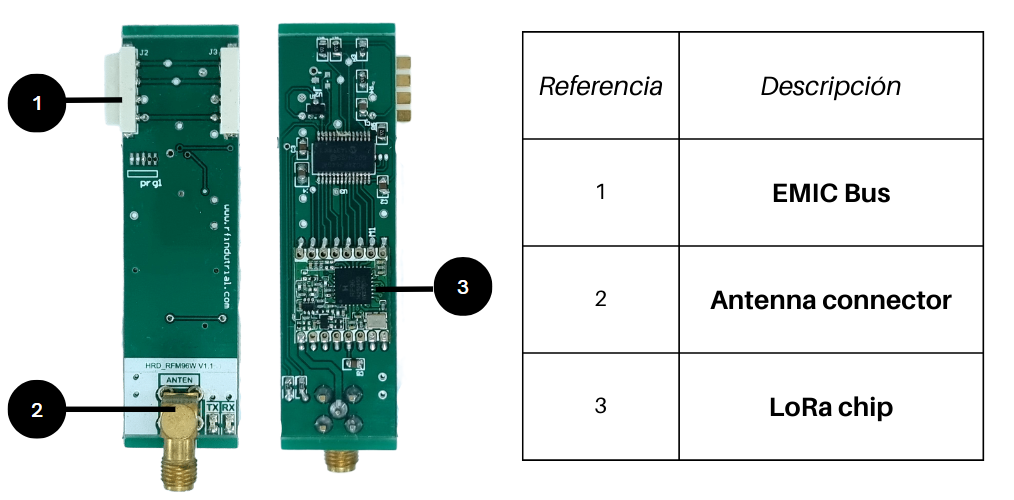
\includegraphics[width=1\textwidth]{./Figures/EMIC-radio-lora.png}
\caption{Esquema de red.}
\label{fig:Hardware}
\end{figure}

\section{Protocolo de enrutamiento}

Un protocolo de enrutamiento de paquetes es un conjunto de reglas y procedimientos que se utilizan para determinar cómo se transmiten los paquetes de datos a través de una red de dispositivos. Estos protocolos permiten que los paquetes sean enviados de manera eficiente desde el origen al destino a través de una serie de nodos intermedios.

El enrutamiento de paquetes implica tomar decisiones sobre la mejor ruta para enviar los paquetes en función de la topología y las condiciones actuales de la red. A continuación se mencionan algunos de las principales problemáticas a ser resueltas por un protocolo de enrutamiento.

\subsection{Descubrimiento de la topología}

El protocolo necesita conocer la estructura y los enlaces de la red para tomar decisiones de enrutamiento. Esto lo logra intercambiando estableciendo los mecanismos necesarios para que los nodos de la red puedan intercambiar información de estado o de enlace.

\subsection{Construcción de la tabla de enrutamiento}

Cada nodo de la red mantiene una tabla de enrutamiento que indica las rutas disponibles hacia diferentes destinos. Esta tabla se crea a partir de la información recopilada durante el descubrimiento de la topología y se actualiza dinámicamente a medida que la red cambia.

\subsection{Selección de la mejor ruta}

Basándose en la información de la tabla de enrutamiento, cada nodo toma decisiones sobre la ruta óptima para enviar los paquetes. Al momento de tomar estas decisiones se pueden considerar una sería de  métricas, como la latencia, el ancho de banda o el costo de los enlaces.

\subsection{Actualización de la información de enrutamiento}

Los protocolos de enrutamiento utilizan diferentes mecanismos para mantener la información de enrutamiento actualizada. Esto puede incluir la difusión periódica de actualizaciones de enrutamiento, el intercambio de mensajes de estado entre nodos adyacentes o la detección de cambios en la topología de la red.

\subsection{Resolución de problemas y enrutamiento alternativo}

Los protocolos de enrutamiento deben manejar situaciones en las que se producen fallas o congestión en los enlaces de la red. Esto implica detectar y resolver problemas de enrutamiento, así como encontrar rutas alternativas cuando una ruta principal no está disponible.

\section{Enrutamiento de vector distancia}

Cada router mantiene una tabla  que contiene información sobre las rutas disponibles y las distancias asociadas a cada destino. La distancia generalmente se mide en términos de saltos o en otras métricas como el costo, el retardo o el ancho de banda.\citep{rip}

\section{Requisitos de la implementación}

Como se ha mencionado anteriormente el proyecto surgió a partir de la necesidad de poder desplegar redes más robustas haciendo uso del módulo "HRD-Radio LoRa". Para esto se buscó desarrollar un protocolo que pudiese ser ejecutado sobre estos dispositivos y pudiera dotar a las redes de una serie de características que se describen en los siguientes párrafos.

Se deberá contemplar la existencia de tres tipos de elementos. Los servidores externos, los nodos finales y los nodos ruteadores.

Los servidores externos representan dispositivos que existen fuera de la red generada con los "HRD-Radio-LoRa". Su función es la de intercambiar datos con los nodos finales.

Los nodos finales son dispositivos que existen dentro de la red generada con los "HRD-Radio-LoRa". Son los encargados de generar los datos destinados a los servidores externos y también cuentan con la capacidad para recibir datos que estos envíen hacia ellos. La mayor parte del tiempo se mantienen en estado de bajo consumo, lo que implica que quedan fuera de la red. Sólo acceden a la red cuando necesitan enviar datos hacia los servidores externos. Una vez que envían esos datos, permanecen durante un tiempo esperando por datos que pudieran llegar de los servidores externos al cabo del cuál vuelven a pasar a estado de bajo consumo.

Los nodos ruteadores son dispositivos que existen dentro de la red generada con los "HRD-Radio-LoRa". Su función es la de trasladar los datos intercambiados entre los nodos finales y los servidores externos. Para esto intercambian con sus pares mensajes con información de ruteo de manera de lograr mantener la información de las rutas a cada destino actualizadas.



